\chapter{Computational Complexity Analysis}
\label{cha:computational_complexity_analysis}

This chapter investigates the computational complexity of the algorithmic problems introduced in our multi-donor kidney exchange model. We formalize the decision versions of these problems and show that they are NP-complete, even under seemingly simple constraints.

We begin by presenting several variants of the problem that differ in the allowed structure of exchanges, such as the maximum length of cycles and chains. We then prove that all of these variants are NP-complete. These results motivate the need for approximation algorithms and heuristic methods, which will be discussed in later chapters.

\section{Problem Variants and Overview of Results}

All problem variants considered in this chapter revolve around structural constraints imposed on the kidney exchange process, specifically, limitations on the maximum length of allowed exchange cycles and chains.

We begin by showing that for any fixed constant $k \ge 2$, the decision version of the \textit{$k$-Cycle Unbounded-Chain Multi-Donor Kidney Exchange Problem} is NP-complete. This result is established via a reduction from the \textit{Longest Path from Fixed Source} problem.

Subsequently, we show that for all $n \in \{n : n \ge 2\} \cup \{\infty\}$ and $m \in \{m:m \ge 1\} \cup \{\infty\}$, \textit{n-Cycle m-Chain Multi-Donor Kidney Exchange Problem} is computationally hard, using a reduction from the \textit{2P2N 3-SAT} problem.



\section{Reduction from Longest Path}

In this section, we formally establish the computational hardness of the matching problems defined in our multi-donor kidney exchange model. Specifically, we show that even under simple structural constraints (such as allowing only one 2-cycle and unrestricted chains) the decision version of the problem remains NP-complete. 

\subsection{NP-Completeness of the 2-Cycle Unbounded-Chain Problem}

\begin{lemma}
The decision version of the \textit{2-Cycle Unbounded-Chain Multi-Donor Kidney Exchange Problem} is NP-complete.
\end{lemma}

\begin{proof}[Proof Sketch]
We prove NP-hardness by reduction from the \textit{Longest Path from Fixed Source} problem (\autoref{prob:longest_simple_path}). Given a directed graph $G = (V, E)$, a designated source node $s$, and an integer $k$, we construct an instance of the \textit{2-Cycle Unbounded-Chain Multi-Donor Kidney Exchange} problem such that there exists a solution saving at least $3 + 2k$ patients if and only if there exists a simple path of length at least $k$ starting from $s$ in $G$.

To construct the kidney exchange instance, we begin by adding a single 2-cycle between two patient-donor groups, where one of the patients is associated with two donors: one donor participates in the 2-cycle, and the other is compatible with the patient corresponding to node $s$ in $G$. This setup initiates the only possible chain in the instance.

Next, for each vertex $v \in V$, we create a corresponding patient-donor pair; $p_v$, $d_v$. For every directed edge $(a, b) \in E$, we introduce a new intermediate patient-donor pair; $p_{ab}$, $d_{ab}$, and add two compatibility edges; $(d_a, p_{ab})$ and $(d_ab, p_b)$. This models each edge as a two-step donation chain segment, as shown in \autoref{fig:longest_path_edge_gadget}.


\begin{figure}
    \centering
    
\includegraphics{data/longest_path_edge_gadget.pdf}
    \caption[Edge gadget used in reduction from Longest Path from Fixed Source problem.]{Edge gadget used in reduction from Longest Path from Fixed Source problem.}
    \label{fig:longest_path_edge_gadget}
\end{figure}


In the resulting kidney exchange instance, only the single 2-cycle we constructed initially is eligible to be selected under the problem constraints. Chains can only be initiated from this 2-cycle and must respect donor compatibility. Since all other potential cycles in the graph (formed via edge constructions) involve at least four patients, no other 2-cycles exist in the instance.

Therefore, maximizing the number of patients who receive a kidney corresponds to finding the longest simple path in $G$ starting from $s$. Each edge in $G$ contributes two transplantations (through the intermediate patient-donor pair), and the initial 2-cycle saves two patients, plus one more as the entry to the chain. Hence, the total number of patients saved is at least $3 + 2k$ if and only if there exists a simple path of length at least $k$ in the original graph.

An example instance of \textit{Longest Path from Fixed Source} problem and its corresponding reduction to the instance of the \textit{2-Cycle Unbounded-Chain Multi-Donor Kidney Exchange} problem is shown in \autoref{fig:longest_path_graph_example}.

\begin{figure}
    \centering
    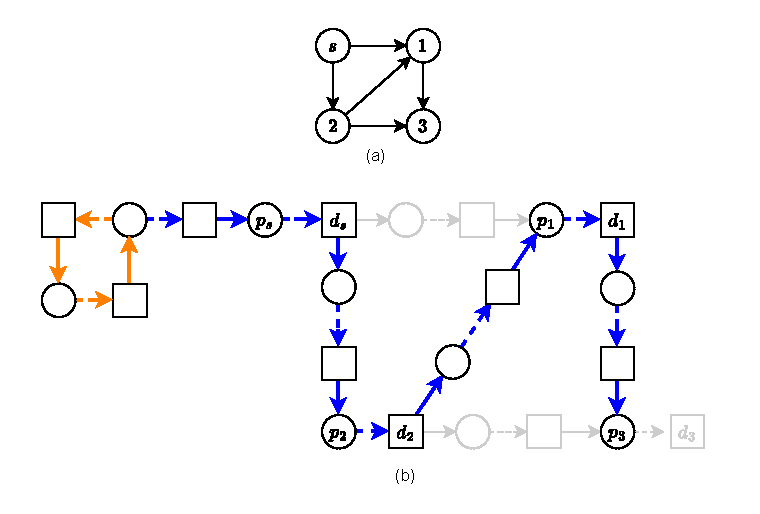
\includegraphics{data/longest_path_graph_example.pdf}
    \caption[An example instance of \textit{Longest Path from Fixed Source} problem and its corresponding reduction to the instance of the \textit{2-Cycle Unbounded-Chain Multi-Donor Kidney Exchange} problem]{\textbf{(a)} shows an example graph instance of \textit{Longest Path from Fixed Source} problem, where the longest path $(s \rightarrow 2 \rightarrow 1 \rightarrow 3)$ has length 3. \textbf{(b)} illustrates the same graph represented in the \textit{2-Cycle Unbounded-Chain Multi-Donor Kidney Exchange} problem and the corresponding optimal solution. The orange 2-cycle on the left initiates the longest available chain consisting of 7 transplantations. The solution sums up to 9 patients saved in total.}
    \label{fig:longest_path_graph_example}
\end{figure}

Membership in NP is immediate, since a proposed matching (i.e., a set of selected cycles and chains) can be verified in polynomial time.
\end{proof}

\subsection{Extensions to $n$-Cycle Constraints}

We now extend the previous hardness result to two broader settings, where the constraint on the length of cycles is generalized from length 2 to an arbitrary constant $n \ge 2$.

\begin{lemma}
For any fixed constant $n \ge 2$, the decision version of the \textit{$n$-Cycle Unbounded-Chain Multi-Donor Kidney Exchange Problem} is NP-complete.
\end{lemma}

\begin{proof}[Proof Sketch]
The proof follows a similar reduction as in the 2-cycle case. At the beginning, we construct a cycle of length $2$ that initiates a chain. 

We ensure that this is the only valid cycle in the constructed. To achieve this, we modify the edge gadgets from the original reduction. Each edge $(a, b)$ is now represented by an expanded chain segment, composed of additional $n$ intermediate patient-donor pairs, such that any cycles formed from these components are of length strictly greater than $n$. This guarantees that under the $n$-Cycle constraint, the only valid cycle is the one we intentionally constructed for initiating the chain.

Thus, as in the 2-cycle case, any feasible solution must rely on a single chain starting from the constructed $n$-cycle. The total number of patients that can be served remains a function of the chain's length, which in turn corresponds to the length of a simple path in the original graph. Therefore, the reduction remains valid for arbitrary fixed $n$.
\end{proof}



\section{Reduction from 2P2N-3SAT}

In the following two lemmas, we show that for all $n \in \{n : n \ge 2\} \cup \{\infty\}$ and $m \in \{m:m \ge 1\} \cup \{\infty\}$, \textit{n-Cycle m-Chain Multi-Donor Kidney Exchange Problem} is computationally hard. This result is established via a reduction from the \textit{2P2N-3-SAT} problem (\autoref{prob:2p2n_3sat}). 

\begin{lemma}
\label{lemma:2c1c_npc}
The decision version of the \textit{2-Cycle 1-Chain Multi-Donor Kidney Exchange Problem} is NP-complete.
\end{lemma}

\begin{proof}[Proof Sketch]
We prove NP-hardness via a reduction from the \textit{2P2N-3-SAT} problem. Let $\phi$ be a Boolean formula in conjunctive normal form, consisting of a set of clauses $C$ and a set of variables $X$, where each clause $c \in C$ contains exactly three literals, and each variable $x \in X$ appears in two clauses as a positive literal $x$ and in two clauses as a negative literal $\neg{x}$. We construct a corresponding instance of the \textit{2-Cycle 1-Chain Multi-Donor Kidney Exchange Problem} such that $\phi$ is satisfiable if and only if there exists a feasible exchange satisfying at least a certain number of patients $t$ (specified below).

In the construction, each clause $c \in C$ is represented as a patient-donor pair $(p_c, d_c)$. For each variable $x \in X$, we construct a special gadget illustrated in \autoref{fig:sat_reduction_boolean_gadget}. The gadget consists of patient-donor groups forming four overlapping cycles and four patient-donor pairs representing two negative literals ($\neg{x}$) and two positive literals ($x$). The gadget is designed so that either the two patients representing the positive literals $p_x$ are satisfied (as shown in \textbf{(b)}), or the two patients representing the negative literals $p_{\neg{x}}$ are satisfied (as shown in \textbf{(c)}), but never both $p_x$ and $p_{\neg{x}}$ simultaneously. The patients representing clauses and those representing literals are the same nodes in our construction. For example, given a clause $c = (x_1, \neg{x_2}, x_3)$, we identify $p_c = p_{x_1} = p_{\neg{x_2}} = p_{x_3}$.

\begin{figure}
    \centering
    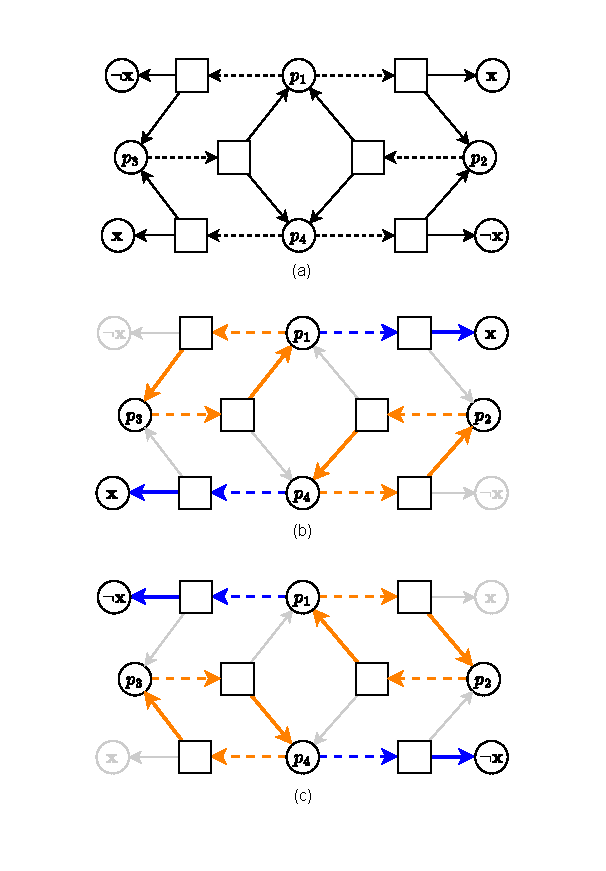
\includegraphics{data/sat_reduction_boolean_gadget.pdf}
    \caption[Boolean variable gadget used in the reduction from \textit{2P2N 3-SAT} to the \textit{2-Cycle 1-Chain Multi-Donor Kidney Exchange Problem}]{Boolean variable gadget used in the reduction from \textit{2P2N 3-SAT} to the \textit{2-Cycle 1-Chain Multi-Donor Kidney Exchange Problem}.\\
    \textbf{(a)} The full variable gadget, representing variable \(x\). \textbf{(b)} An assignment where the variable is set to \texttt{true}, \textbf{(c)} An assignment where the variable is set to \texttt{false}. Only one of these two assignments can be selected in a valid matching, ensuring that either \(x\) or \(\neg{x}\) is selected, but not both.}\label{fig:sat_reduction_boolean_gadget}
\end{figure}

In \autoref{fig:sat_reduction_boolean_gadget}, notice that no matter which pair of cycles is selected, the four patients $p_1$, $p_2$, $p_3$, and $p_4$ always receive compatible kidneys. If $\phi$ is satisfiable, then in our construction all patients representing clauses ${ p_c : c \in C }$ receive compatible kidneys in every optimal solution. Conversely, if $\phi$ is not satisfiable, then in every solution there exists at least one patient representing a clause who does not receive a compatible kidney. This gives rise to the threshold $t = 4 \cdot |X| + |C|$, indicating that the solution to the constructed instance of the \textit{2-Cycle 1-Chain Multi-Donor Kidney Exchange Problem} satisfies $t$ patients if and only if $\phi$ is satisfiable.

The problem is clearly in NP. Given a proposed solution to the instance of the \textit{2-Cycle 1-Chain Multi-Donor Kidney Exchange Problem}, we can verify in polynomial time whether it satisfies at least $t = 4 \cdot |X| + |C|$ patients. 

Since the problem is both in NP and NP-hard, we conclude that the decision version of the \textit{2-Cycle 1-Chain Multi-Donor Kidney Exchange Problem} is NP-complete.
\end{proof}


\begin{lemma}
\label{lemma:ncmc_npc}
For all $n \in \{n : n \ge 2\} \cup \{\infty\}$ and $m \in \{m:m \ge 2\} \cup \{\infty\}$, The decision version of the \textit{n-Cycle m-Chain Multi-Donor Kidney Exchange Problem} is NP-complete.

\begin{proof}[Proof Sketch]
This proof is almost identical to the one of \autoref{lemma:2c1c_npc}. What changes is the structure of the variable gadget and the threshold $t$. This time the variable gadget consists of two overlapping cycles of length two, which only one of can be selected. Each of the cycles, when selected, start a donation chain of length two, that can satisfied up to two patients representing positive literals $p_x$ or up to two patients representing negative literals $p_{\neg{x}}$, as it is shown in \textbf{(a)} and \textbf{(b)}. Notice, that in this construction, there are no other cycles and no other chains than the ones just mentioned. That implies, the gadget works for arbitrary values of $n \in \{n : n \ge 2\} \cup \{\infty\}$ and $m \in \{m : m \ge 2\} \cup \{\infty\}$, since only 2-cycles and chains of length 2 are required to encode the variable gadget and satisfy the literals.

The clause gadgets remain unchanged from the previous proof. As before, each clause $c \in C$ is represented by a patient-donor pair $(p_c, d_c)$. Thus, a clause is satisfied in the exchange if and only if it gets a  kidney from one of the associated variable gadgets.

The correctness of the reduction follows similarly: if the Boolean formula $\phi$ is satisfiable, then there exists a consistent assignment of truth values to the variables such that, for each variable $x$, we select the cycle corresponding to either the positive or the negative assignment. This initiates chains satisfying the corresponding literals (and in turn the clauses, since a clause and its corresponding literals are represented by the same patient). As a result, all patients corresponding to clauses receive compatible kidneys, reaching the threshold $t = 3 \cdot |X| + |C|$.

Conversely, if $\phi$ is not satisfiable, then for every selection of variable gadgets, at least one clause cannot be satisfied—meaning its corresponding patient does not receive a kidney. Therefore, the threshold $t$ cannot be reached, and no feasible exchange meets the requirement.

Hence, the decision version of the \textit{n-Cycle m-Chain Multi-Donor Kidney Exchange Problem} is NP-complete for all $n \ge 2$ and $m \ge 2$, including the unbounded cases.

\begin{figure}
    \centering
    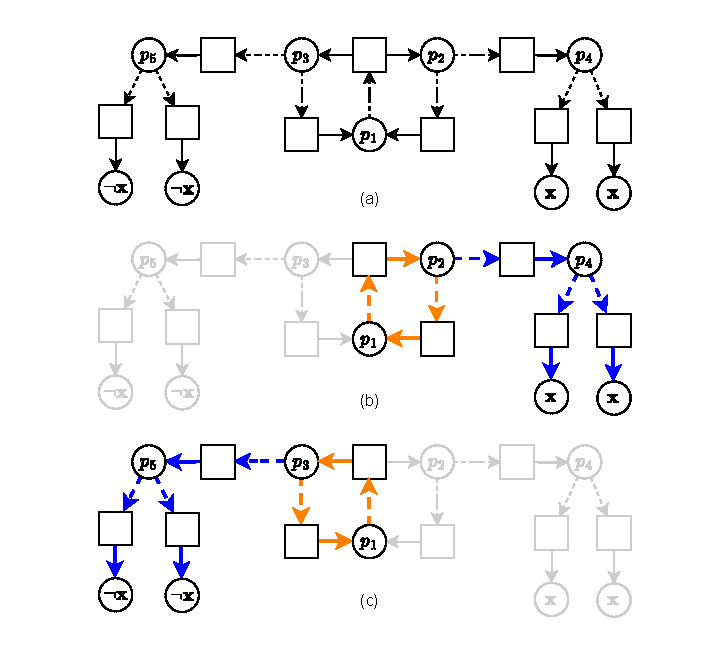
\includegraphics{data/sat_reduction_boolean_gadget2.pdf}
    \caption[Boolean variable gadget used in the reduction from \textit{2P2N 3-SAT} to the \textit{$n$-Cycle $m$-Chain Multi-Donor Kidney Exchange Problem}]{Boolean variable gadget used in the reduction from \textit{2P2N 3-SAT} to the \textit{$n$-Cycle $m$-Chain Multi-Donor Kidney Exchange Problem}.\\
    \textbf{(a)} The full variable gadget, representing variable \(x\). \textbf{(b)} and \textbf{(c)} are assignments where the variable is set to \texttt{true} and \texttt{false} respectively.}\label{fig:sat_reduction_boolean_gadget2}
\end{figure}

\end{proof}
\end{lemma}



%%% Local Variables:
%%% mode: latex
%%% TeX-master: "../ClassicThesis"
%%% ispell-dictionary: "british" ***
%%% fill-column: 76 ***
%%% End:
